% ----------------------------------------------------------------------------
% Apresentação
% ----------------------------------------------------------------------------
 
\chapter{Apresentação}

O Pure Data á um ambiente visual de programação musical que permite criarmos
aplicações musicais complexas a partir da combinação de componentes visuais.
Apesar do Pure Data conter vários componentes prontos há a possibilidade de
criarmos novos objetos em C/C++. Estes objetos são chamados de externals.

Este é um tutorial prático para escrita de externals em C para o Pure Data. A
iniciativa de escrever tal documento surgiu na disciplina de Computação
Musical do Instituto de Matemática e Estatísticas da Universidade de São Paulo
no primeiro semestre de 2011 ministrada pelo professor Marcelo Gomes de
Queiroz. A intenção deste tutorial é tentar auxiliar programadores a
desenvolver externals de maneira bastante simples.

Mais do que ampliar a gama de objetos do Pure Data e criar novos objetos, o
objetivo deste trabalho é também permitir ao pesquisador de computação musical
a implementação e testes de algoritmos de processamento de áudio para caráter
de estudo. Isto significa que podemos reimplementar várias coisas que já
existem no Pure Data simplesmente porque é didático programar e colocar
algoritmos para funcionar.

\section{Escrevendo seus externals}

O Pure Data possui uma API para o desenvolvimento de externals. Para utilizar
esta API é necessário importar a biblioteca m\_pd.h que está disponível em
(http://compbio.cs.toronto.edu/repos/snowflock/mpich-1.2.7/mpid/mpd/mpd.h). Há
um tutorial para escrever externals feito pelo IOHannes, um dos programadores
do Pure Data. Este tutorial está disponível em
http://iem.at/pd/externals-HOWTO/pd-externals-HOWTO.pdf. Apesar deste
documento ter sido meu ponto de partida, boa parte do que contém no presente
tutorial foi aprendido lendo código-fonte de externals do repositório do
próprio Pure Data
(http://pure-data.svn.sourceforge.net/viewvc/pure-data/trunk/externals/).

\section{Organizando seus externals}

É praxe que o arquivo do external tenha o mesmo nome que o external. Se
fossemos fazer, por exemplo, um trigger, o mesmo estaria em um arquivo chamado
trigger.c e seria compilado em um external chamado trigger.pd\_linux ou
trigger.dll ou trigger.pd\_irix5 ou trigger.pd\_darwin. Isto não é obrigatório
mas é uma convenção que facilita a busca do código-fonte deste external no
repositório.

\section{Compilando seus externals}

Um external precisa ser compilado e depois linkado como external. A versão
Linux pode ser feita com os comandos:

\begin{lstlisting}
cc -DPD -O2 -fPIC -funroll-loops -fomit-frame-pointer 
	-Wall -W -Wshadow -Wstrict-prototypes -Werror 
	-Wno-unused -Wno-parentheses -Wno-switch 
	-o example1.o -c example1.c
ld -export_dynamic  -shared -o example1.pd_linux 
	example1.o -lc -lm
rm example1.o
\end{lstlisting}

Para compilar, o ideal é criarmos um Makefile. Todas as pastas de exemplos
deste tutorial estão acompanhadas de um makefile feito pelo Marcelo Queiroz.

\section{Criando help para seus externals}

O arquivo de help deve ter o mesmo nome que o external. Por exemplo, para o
exemplo1.c com o objeto exemplo1 temos o arquivo example1-help.pd. Este
arquivo do puredata com exemplo deve acompanhar o external na instalação,
ficando na mesma pasta que o external compilado.  Há a possibilidade de
associarmos a cada external outros arquivos que não sigam esta convenção e a
mesma será apresentada no próximo capítulo.

\section{Executando seu external}

Se você executar o Pure Data na mesma pasta aonde está seu external compilado,
o mesmo irá funcionar. Caso não esteja executando o pure data via terminal
deverá colocar a pasta aonde o external se encontra no caminho de busca do
Pure Data.

\begin{figure}[h!]
	\centering
	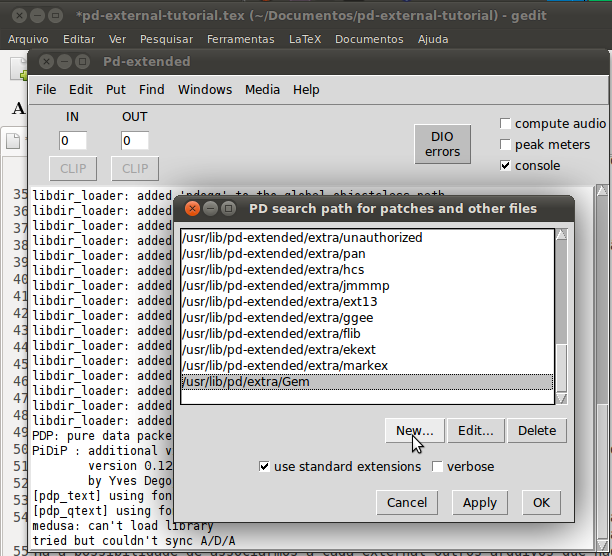
\includegraphics[width=0.7\textwidth]{path}
	\caption{Adicionando o diretório do seu external no Pure Data.}
\end{figure}

Para carregar uma biblioteca de externals (mais de um external no mesmo
arquivo-fonte), é necessário adicionar a biblioteca no Pure Data:

\begin{lstlisting}
pdextended  -lib medusa medusa-help.pd 
\end{lstlisting}

Ou 

\begin{figure}[h!]
	\centering
	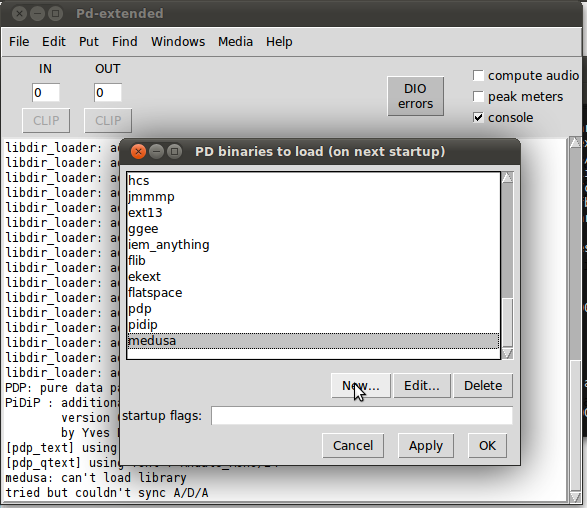
\includegraphics[width=0.7\textwidth]{startup}
	\caption{Adicionando sua biblioteca no Pure Data.}
\end{figure}


